\documentclass[12pt]{article}
\usepackage{../../../assignment}
\usepackage{../../../math}
\usepackage{../../../uark_colors}
\hypersetup{
  colorlinks = true,
  allcolors = ozark_mountains,
  breaklinks = true,
  bookmarksopen = true
}
\newcommand{\answer}[1]{{\color{blue_winged_teal}\textbf{Answer:} #1}}
\newcommand{\pts}[1]{{\color{zinc500} [#1 pts]}}

\begin{document}
\begin{center}
  {\Huge\bf Midterm - Fall 2025}

  \smallskip
  {\large\it ECON 5783 — University of Arkansas}
\end{center}

\medskip
\begin{enumerate}
  \item Say a researcher wants to model the conditional expectation
    of European soccer team performance given total annual player
    salary and country.
    \begin{enumerate}[label=(\alph*)]
      \item \pts{10} They regress 10-year win percentage on a set of indicator
        variables for each European country and a linear term for
        total salaries paid.
        Give two limitations of this model 

      \answer{
        Linearity of total salaries assumes the marginal returns to salaries is constant.
        Second, they do not include interaction between countries and salaries imposing the marginal effect of salaries is the same for each country.
      }
    \end{enumerate}

  \bigskip\bigskip
  \item A researcher wants to estimate the effect of taking vitamin
    supplements on health outcomes.

    \begin{enumerate}[label=(\alph*)]
      \item \pts{10} Do you think the difference-in-means estimate will
        identify the causal effect of supplements?
        If not, predict the sign selection bias and explain your thinking.

      \answer{
        There are many possible answers, but e.g. people that take supplements probably care more about their health and take many actions to improve their health. 
        So even in the absence of the vitamins, the untreated outcomes of the vitamin takers would be higher, biasing the estimates upwards. 
      }

      \item \pts{10} The researchers are aware of this problem and therefore
        use a selection on observables identification strategy.
        They condition on age and self-reported diet quality.
        Describe in your own words what the conditional independence
        assumption is assuming here

      \answer{
        For individuals of the same age and the same self-reported diet quality, whether or not they take a vitamin is as good as randomly assigned (unrelated to other drivers of healt outcomes).
      }

      \item \pts{5} Give an example of why the causal assumption might fail.
      
      \answer{
        This assumption could fail, for example, if supplement use is (negatively) correlated with alcohol consumption and (positively) correlated with exercise, even conditional on age and diet.
      }

      \item \pts{10} Assume that you think the \emph{causal} assumption holds.
        For each of the following estimation strategies, write what a
        researcher needs to worry about: (i) regression adjustment,
        (ii) inverse probability of treatment weighting, (iii)
        aggregating sub-sample ($\bm{X}_i = \bm{x}$) difference-in-means

      \answer{
        (i) Regression adjustment assumes correct modeling of the potential outcomes as a function of $\bm{X}$. 
        (ii) IPTW assumes correct modeling of the propensity as a function of $\bm{X}$. 
        (iii) sub-sample difference-in-means suffers from the curse of dimensionality when the dimension of $\bm{X}$ is large.
      }        
    \end{enumerate}
\end{enumerate}

\newpage
\noindent
% https://arxiv.org/pdf/2508.02658v1
The following questions refer to new work by Feng and Ruggieri (2025).
These authors use a regression discontinuity design to estimate the
housing price effect of school district finance referendums passing.
They look at narrowly winning and narrowly losing elections on home
prices 5 years later (to allow time for capitalization).
See the following figure for their main estimate

\begin{figure}[!b]
  \centering
  \caption{RDD Estimates}
  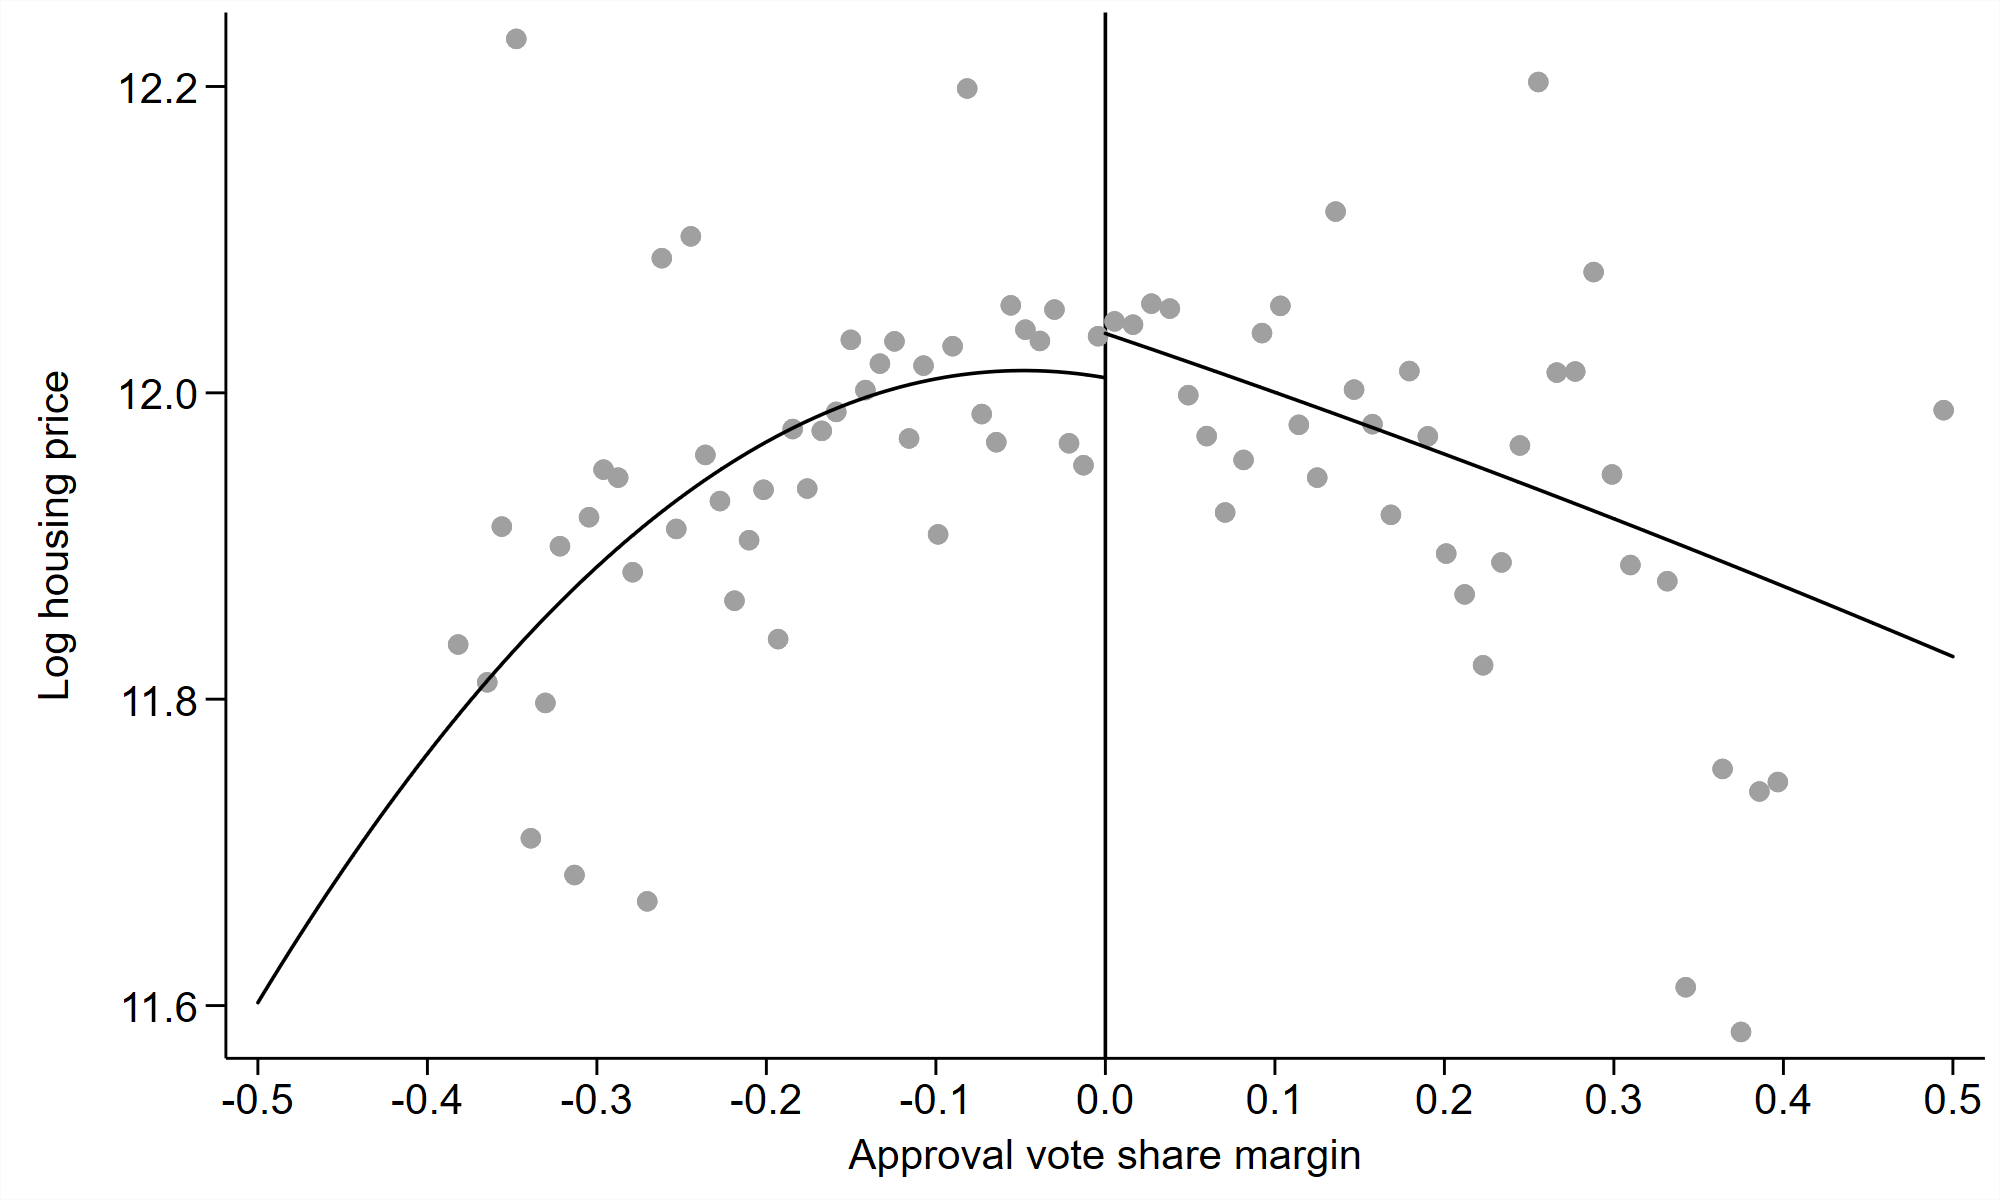
\includegraphics[width=0.85\textwidth]{Feng_Ruggieri_2025.png}
\end{figure}

\begin{enumerate}
    \setcounter{enumi}{2}
  \item \pts{10} What do the authors need to assume for the RDD estimate to be
    interpreted as causal?
    Argue why this might be plausbile in the context of referendum vote share.

  \answer{
    The authors need to assume continuity of potential outcomes at the cut-off (i.e. no sorting or manipulation of the vote share). 
    In the context of referendum vote share, this is reasonable since places that just narrowly approve and just narrowly reject the referendum probably look very similar. 
    More, it is very difficult to precisely manipulate vote-share.
  }

  \item \pts{10} The authors do not include data for referendum that are
    raised multiple years in a row by the same district.
    Why might including those elections create problems with the
    causal assumption you discussed in the previous question?

  \answer{
    Places that try to pass the referendum multiple times until they succeed create an issue of sorting at the cutoff. 
    The places that do this might differ than places that give up after the first failure, creating a discontinuity in outcomes at the cut-off.
  }

  \item \pts{5} In class we discussed that RDD identifies the LATE (Local
    ATE) for disctricts at the 50\% vote cutoff.
    Given this, why might we think the effects for this group differ
    from districts where the referendum passes by large margins.

  \answer{
    The LATE that is identified by the RDD will be in the kinds of places that marginally support schools.
    These places might have smaller treatment effects than places where they value school spending more (e.g. if school spending and parental involvement are complements).
  }
\end{enumerate}

\newpage
\noindent
The following questions refer to the paper Systemic Discrimination
Among Large U.S. Employers by Kline, Rose, and Walters (2022, QJE).
The authors ran a large-scaled randomized experiment `sending more
than 83,000 fictitious applications with randomized characteristics
to geographically dispersed jobs posted by 108 of the largest U.S. employers.'
For each application, they randomly changed the applicant to have
`distinctivly Black' or `disctinctivly White' names.
They find that on avereage `Distinctively Black names reduce the
probability of employer contact by 2.1 percent-age points relative to
distinctively white names.'

\bigskip
\begin{enumerate}
    \setcounter{enumi}{5}
  \item \pts{10} Say the authors instead only had a non-experimental sample of
    workers' applications and whether or not they received an employer callback.
    Why might the difference in callback rate between Black and White
    workers not be completely explained as the ``causal discriminatory effect''?

    \answer{
      Black and White candidates might differ in many ways (e.g. differences in education, experience, or other background characteristics).
    }

  \item \pts{10} The authors include table 1 in the paper summarizing
    information from the applications they send.
    Why do you think they include this table?

  \answer{
    The authors include table 1 to highlight the the applications they sent looked very similar for each group. 
    This helps control for other differences in applicants and isolates the `discrimination effect'. 
    The table validates the randomization of names.
  }

  \item \pts{10} The paper then tries to estimate firm-specific discrimination
    estimates (firm-specific difference in callback rate).
    This results in many different "small experiments" for each individual firm.
    Say a newspaper wanted to take the estimates from this and label
    `the 5 most discriminatory firms'.
    Why might you caution this reporter of selecting the most
    discriminatory estimates?

  \answer{
    Since each firm estimate is quite noisy, we face the issue of selecting based on noise.
    The firms with the highest estimates might not be the most discriminating firms (the so-called `winners curse').
  }
\end{enumerate}

\begin{table}[!b]
  \centering
  \caption{Characteristics of Applications}
  \begin{tabular}{lccc}
    \toprule
    & {\small`Distinctively White' } & {\small`Distinctively Black' Names} & \\
    & {\small Names} & {\small Names} & {\small Difference} \\
    \midrule
    Résumé characteristics \\
    \quad Female & $0.500$ & $0.498$ & $0.003$ \\
    \quad Over 40 & $0.534$ & $0.533$ & $0.002$ \\
    \quad LGBTQ club member & $0.079$ & $0.080$ & $-0.001$ \\
    \quad Academic club & $0.039$ & $0.042$ & $-0.003^{*}$ \\
    \quad Political club & $0.042$ & $0.041$ & $0.001$ \\
    \quad Gender-neutral pronouns & $0.040$ & $0.040$ & $0.000$ \\
    \quad Same-gender pronouns & $0.042$ & $0.041$ & $0.001$ \\
    \quad Associate degree & $0.478$ & $0.485$ & $-0.006^{*}$ \\
    \bottomrule
  \end{tabular}
\end{table}

\end{document}
